%\documentclass[12pt,english]{article}
%\usepackage{fullpage}
%\usepackage[T1]{fontenc} 
%\usepackage{helvet}
%\renewcommand{\familydefault}{\sfdefault}
%\usepackage{babel}
%\usepackage{amsmath}
%\numberwithick{equation}{section}
%\usepackage{hyperref}
%\usepackage{tikz,pgfplots}
%\usepackage{boldline} %To get thicker lines in tables
%\usepackage{float}    %For float on figures for exampel
%\usepackage{graphicx} %Figures
%
%\usepackage{sectsty}
%\allsectionsfont{\centering}
%
%\renewcommand{\thesubsection}{\Roman{subsection}} 
%\renewcommand{\thesubsubsection}{\Alph{subsubsection}} 
%
%\newcommand{\ignore}[1]{}
%\def\circledarrow#1#2#3{ % #1 Style, #2 Center, #3 Radius
%  \draw[#1,->] (#2) +(80:#3) arc(80:-260:#3);
%}
%
%\begin{document}
%
%\begin{figure}[H]
%  \centering
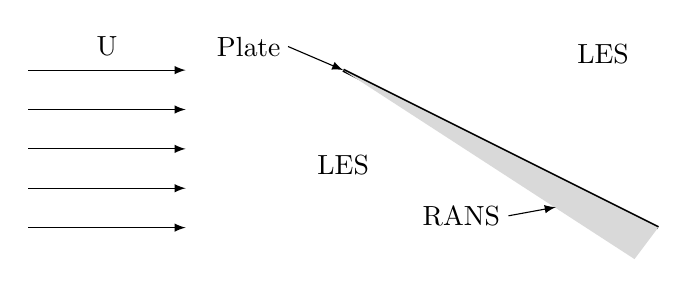
\begin{tikzpicture}
  \coordinate (A) at (0,0);
  \coordinate (B) at (2,0);
  \coordinate (C) at (0,0.5);
  \coordinate (D) at (2,0.5);
  \coordinate (E) at (0,1);
  \coordinate (F) at (2,1);
  \coordinate (G) at (0,1.5);
  \coordinate (H) at (2,1.5);
  \coordinate (I) at (0,2);
  \coordinate (J) at (2,2);
  %Arrows
  \draw[-latex] (A)--(B);
  \draw[-latex] (C)--(D);
  \draw[-latex] (E)--(F);
  \draw[-latex] (G)--(H);
  \draw[-latex] (I)--(J);
  %Plates
  \coordinate (AA) at (4,2);
  \coordinate (BB) at (8,0);
  \coordinate (CC) at (7.7,-0.4);
  \draw[very thick] (AA)--(BB);
  \fill[gray!30] (AA) -- (BB) -- (CC) -- cycle;
  %circles - First
  \circledarrow{thick, gray}{4.3,2}{0.1cm};
  \circledarrow{thick, gray}{4.65,1.95}{0.1cm};
  \circledarrow{thick, gray}{4.95,1.7}{0.1cm};
  \circledarrow{thick, gray}{5.4,1.5}{0.1cm};
  \circledarrow{thick, gray}{5.9,1.3}{0.1cm};
  \circledarrow{thick, gray}{6.3,1.1}{0.1cm};
  \circledarrow{thick, gray}{6.7,0.95}{0.1cm};
  \circledarrow{thick, gray}{7.1,0.7}{0.1cm};
  \circledarrow{thick, gray}{7.5,0.5}{0.1cm};
  \circledarrow{thick, gray}{8.0,0.3}{0.1cm};
  %Circles - second
  \circledarrow{thick, gray}{5.2,1.85}{0.15cm};
  \circledarrow{thick, gray}{5.7,1.7}{0.15cm};
  \circledarrow{thick, gray}{6.2,1.5}{0.15cm};
  \circledarrow{thick, gray}{6.6,1.3}{0.15cm};
  \circledarrow{thick, gray}{6.9,1.8}{0.15cm};
  \circledarrow{thick, gray}{7.2,1.0}{0.15cm};
  \circledarrow{thick, gray}{7.8,0.8}{0.15cm};
  \circledarrow{thick, gray}{8.2,0.95}{0.15cm};
  %Circle - third
  \circledarrow{thick, gray}{6.4,1.9}{0.2cm};
  \circledarrow{thick, gray}{7.0,1.45}{0.2cm};
  \circledarrow{thick, gray}{7.5,1.6}{0.2cm};
  \circledarrow{thick, gray}{7.8,1.2}{0.2cm};
  \circledarrow{thick, gray}{8.3,1.5}{0.2cm};
  
  \node at (1,2.3) {U};
  \node at (4,0.8)  {LES};
  \node at (7.3,2.2)  {LES};
  \node at (5.5,0.15) {RANS};
  \node at (2.8,2.3)  {Plate};

  \draw [-latex] (3.3,2.3)--(4.0,2.0);
  \draw [-latex] (6.1,0.15)--(6.7,0.26);
  %\draw[step=0.1cm,gray,very thick] (4,0) grid (9,2);

\end{tikzpicture}
%  \caption{???}
%  \label{fig:zones}
%\end{figure}
%\end{document}
